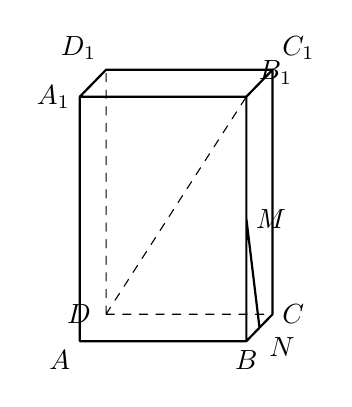
\begin{tikzpicture}[line cap=round,line join=round,x=0.9cm,y=0.9cm]
  \coordinate (A) at (0,0);
  \coordinate (B) at (2.35,0);
  \coordinate (C) at (2.72,0.38);
  \coordinate (D) at (0.37,0.38);
  \coordinate (Aone) at (0,3.45);
  \coordinate (Bone) at (2.35,3.45);
  \coordinate (Cone) at (2.72,3.83);
  \coordinate (Done) at (0.37,3.83);
  \coordinate (M) at (2.35,1.725);
  \coordinate (N) at (2.535,0.19);

  % Rear-left and rear-bottom edges are hidden; B_1D is hidden inside the prism.
  \draw[dashed] (D)--(C) (D)--(Done) (D)--(Bone);
  \draw[thick] (A)--(B)--(C) (A)--(Aone)--(Bone)--(Cone)--(Done)--(Aone)
               (B)--(Bone) (C)--(Cone) (M)--(N);

  \node[below left] at (A) {$A$};
  \node[below] at (B) {$B$};
  \node[right] at (C) {$C$};
  \node[left=2pt] at (D) {$D$};
  \node[left] at (Aone) {$A_1$};
  \node[above right=1pt] at (Bone) {$B_1$};
  \node[above right] at (Cone) {$C_1$};
  \node[above left] at (Done) {$D_1$};
  \node[right] at (M) {$M$};
  \node[below right] at (N) {$N$};
\end{tikzpicture}
